\documentclass[aspectratio=169]{beamer}

\usepackage[utf8]{inputenc}
\usetheme{default}
\setbeamertemplate{navigation symbols}{}
\setbeamertemplate{footline}[frame number]

\title{Dranspose}
\subtitle{A constrained map-reduce live analysis pipeline for fast experimental feedback}
\author{Felix Engelmann, Scientific Data \\\medskip \url{fe-research@nlogn.org}}
\date{25$^\text{th}$ September 2024}


% TODO: table for use cases
% TODO: fix trigger map

\usepackage{appendixnumberbeamer}

\usepackage{tabularx}
\usepackage{array}
\usepackage{tikz}
\usepackage{fontawesome5}

\usepackage{pgfplots}

\pgfplotsset{compat=1.14}
\usetikzlibrary{pgfplots.groupplots}

\DeclareFixedFont{\ttb}{T1}{txtt}{bx}{n}{12} % for bold
\DeclareFixedFont{\ttm}{T1}{txtt}{m}{n}{12}  % for normal

% Custom colors
\usepackage{color}
\definecolor{deepblue}{rgb}{0,0,0.5}
\definecolor{deepred}{rgb}{0.6,0,0}
\definecolor{deepgreen}{rgb}{0,0.5,0}

\usepackage{listings}

% Python style for highlighting
\newcommand\pythonstyle{\lstset{
language=Python,
basicstyle=\ttm,
morekeywords={self},              % Add keywords here
keywordstyle=\ttb\color{deepblue},
emph={EventData, StreamData,__init__},          % Custom highlighting
emphstyle=\ttb\color{deepred},    % Custom highlighting style
stringstyle=\color{deepgreen},
%frame=tb,                         % Any extra options here
showstringspaces=false
}}


% Python environment
\lstnewenvironment{python}[1][]
{
\pythonstyle
\lstset{#1}
}
{}

\begin{document}
\begin{frame}
\titlepage
\end{frame}




\begin{frame}{Experimental Feedback Loop}
 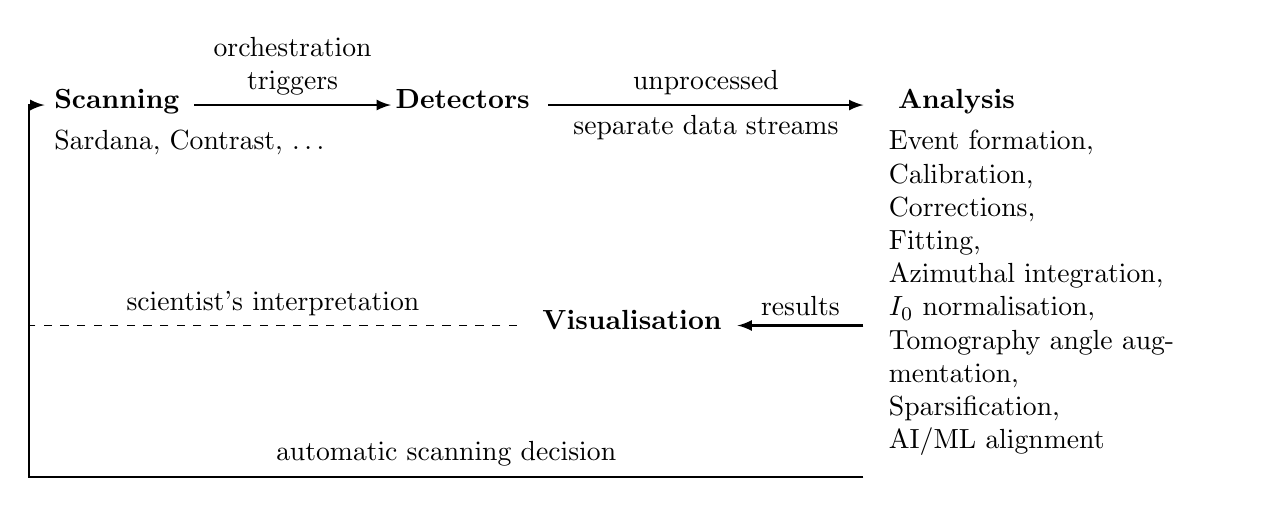
\begin{tikzpicture}[xscale=0.2,yscale=0.8]
 \node[below right, text width=15cm] (sc) at (-1,-0.9) {\textbf{Scanning}\\[1mm]
 Sardana, Contrast, \dots};

 \node[text width=4cm, below right] at (52,-0.9) {\textbf{ Analysis}\\[1mm]
   Event formation,\\
   Calibration, \\
   Corrections, \\
   Fitting, \\
   Azimuthal integration, \\
   $I_0$ normalisation,\\
   Tomography angle augmentation, \\
   Sparsification,\\
   AI/ML alignment};

 \node[below right] at (30,-4.4) {\textbf{Visualisation}};

 \node[below right] (det) at (20,-0.9) {\textbf{ Detectors}};

 \draw[-latex, thick] (8.5,-1.3) -- node[above, text width=3cm, align=center]{ orchestration\\
 triggers} +(12.5,0);
 \draw[-latex, thick] (31,-1.3) -- node[above]{ unprocessed} node[below]{ separate data streams} +(20,0);

 \draw[-latex, thick] (51,-4.8) -- node[above]{results} +(-8,0);

 \draw[dashed] (29,-4.8) -| node[near start, above]{scientist's interpretation} (-2,-3.5);

 \draw[-latex,thick] (51,-7.2) -| node[near start, above]{automatic scanning decision} (-2,-3.5) |- (-1,-1.3);

\end{tikzpicture}
\end{frame}




\begin{frame}{Most Existing Infrastructure}
\centering
 \begin{tikzpicture}
  \fill[red!20!white] (-0.3,0.3) rectangle (1.7,-3.3);
  \fill[blue!20!white] (3.7,0.3) rectangle (1.7,-3.3);
  \fill[green!20!white] (3.7,0.3) rectangle (6.3,-3.3);
  \node at (-2,0) {Detectors};
  \node (det1) at (0,0) {\faCamera};
  \node (mot) at (4,0) {\faSlidersH}; %\faCameraRetro};
  \node (temp) at (6,0) {\faThermometerHalf};
  \node (det2) at (2,0) {\faVideo};

  \node at (-2,1) {Trigger Source};

  \node (panda) at (0,1) {\faWaveSquare};

  \draw[dotted] (panda) -- (det1);
  \draw[dotted] (panda) -- (det2.north);
  \draw[dotted] (panda) -- (mot.north);
  \draw[dotted] (panda) -- (temp.north);

  \node at (-2,-3) {File Recording};
  \node (file1) at (0,-3) {\faFileImage};
  \node (file2) at (2,-3) {\faFileImage};
  \node (file) at (5,-3) {\faFileArchive};

  \draw[very thick] (det1) -- (file1);
  \draw[very thick] (det2) -- (file2);

  \draw (mot) -- (file);
  \draw (temp) -- (file);

  \node at (-2,-2) {Live Analyses};
  \node (crop) at (0.5,-2) {\faCrop};

  \node at (-2,-4) {Post Analysis};
  \node (ana) at (3,-4) {\faChartArea};

  \draw (file1) -- (ana);
  \draw (file2) -- (ana);
  \draw (file) -- (ana);

  \node at (-2,-1) {Live Viewers};
  \node (live1) at (0.5,-1) {\faDesktop};
  \node (live2) at (2.5,-1) {\faDesktop};


  \draw (det2) -- (live2);

  \node (proc1) at (1.4,-2) {\faDesktop};
  \draw (det1) -- (live1) -- (crop) -- (proc1);

 \end{tikzpicture}

\end{frame}


\begin{frame}{Limitations of Live Analysis}
 \begin{block}{Single Data Stream}
  \begin{itemize}
   \item only one detector data available
   \item simple tools, e.g. azint, crop, time integration
\medskip

   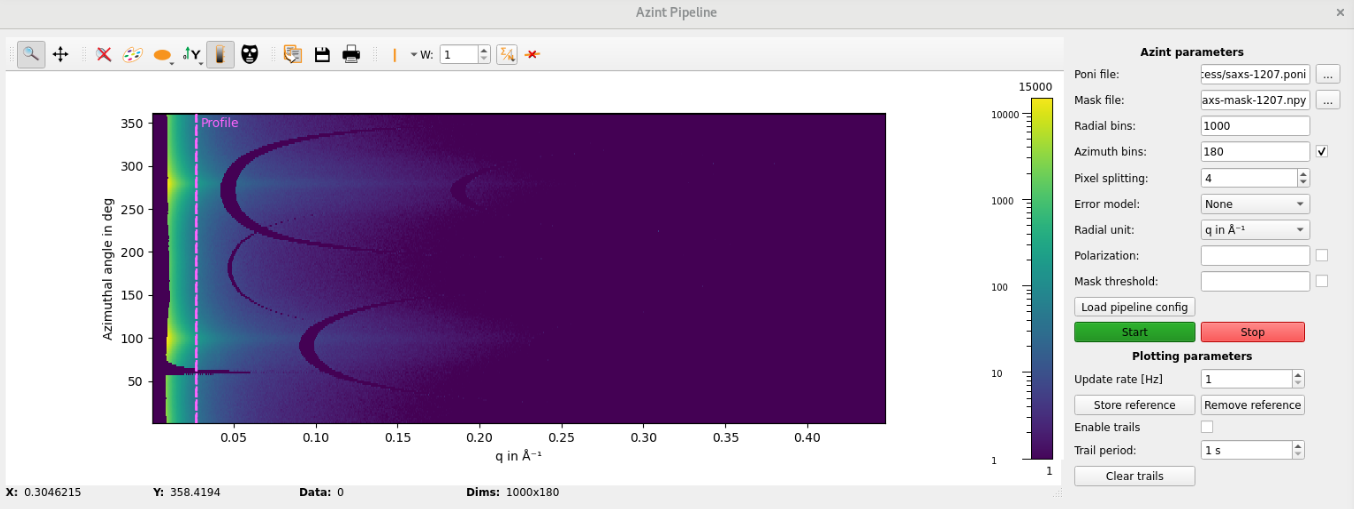
\includegraphics[height=2.7cm]{dets/azint}  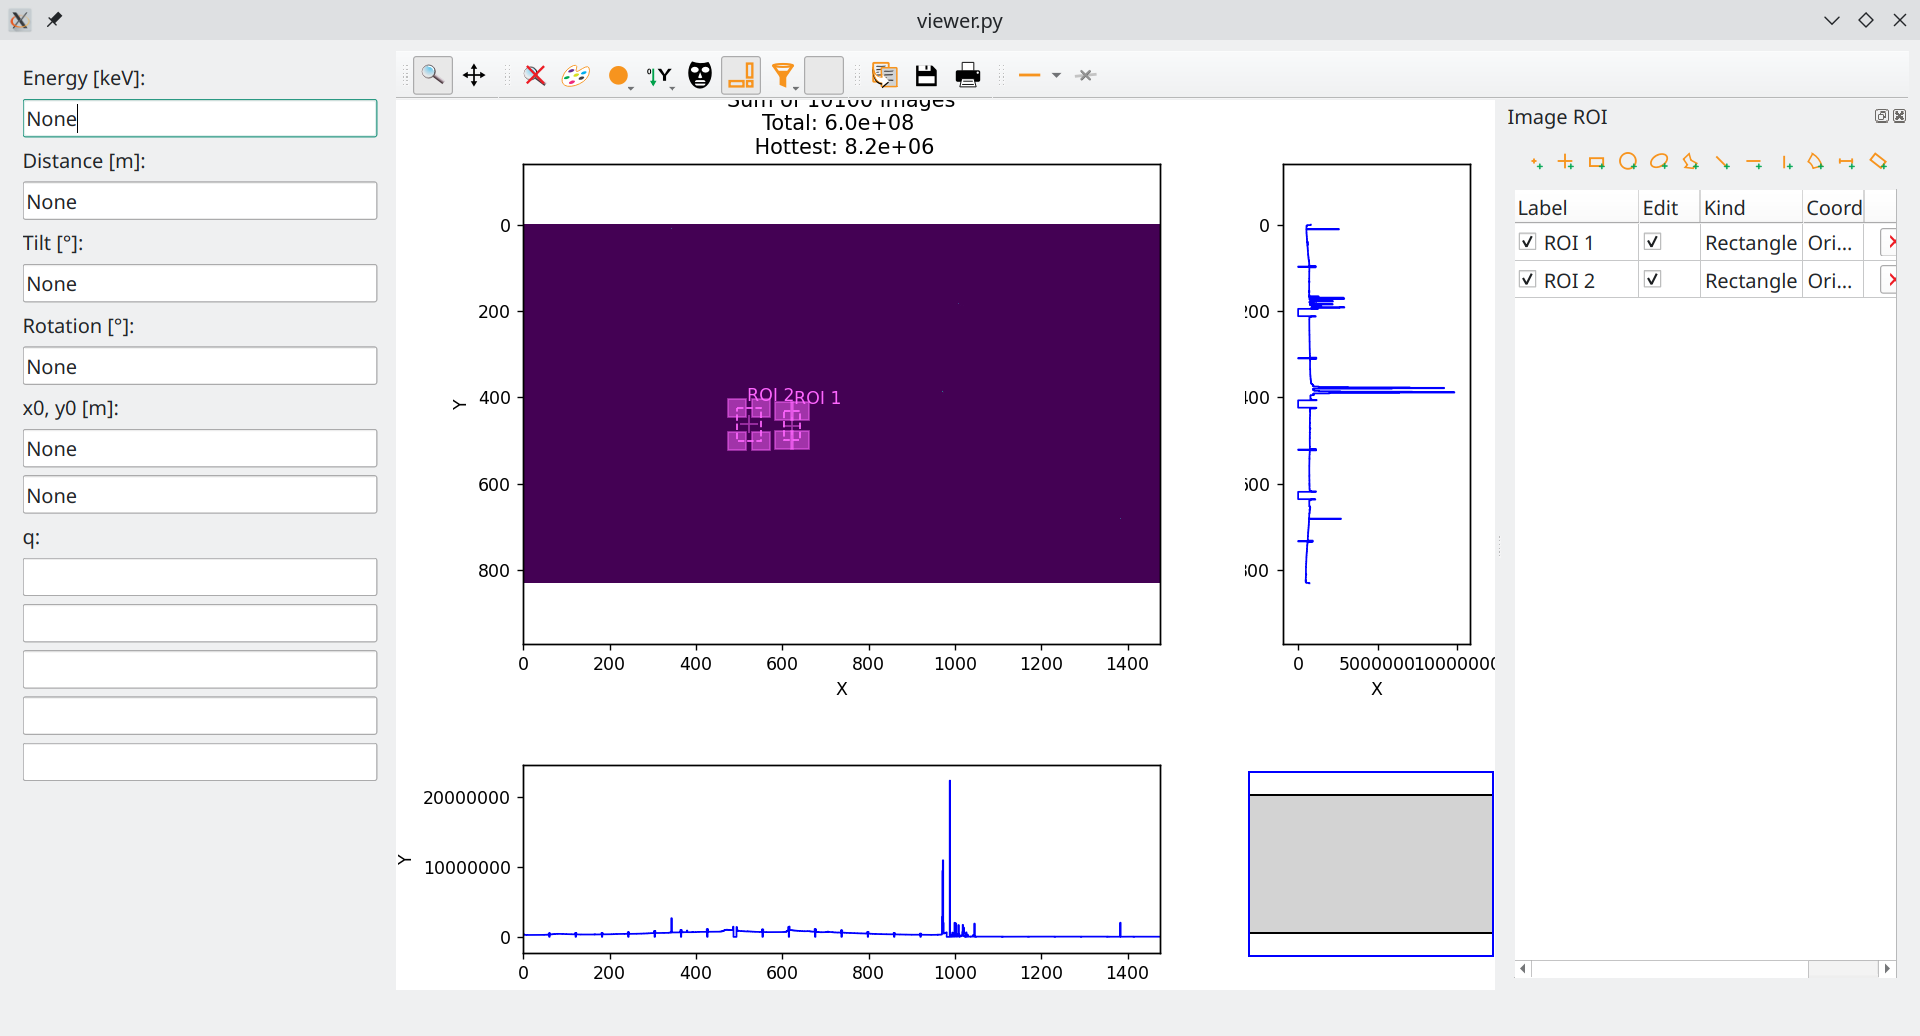
\includegraphics[height=2.7cm]{img/femtomax}
  \end{itemize}
 \end{block}
 \begin{block}{Beyond Limits}
  normalisation to $I_0$, sorting by motor position
 \end{block}
\end{frame}

\begin{frame}{Additional Data Sources}

\begin{minipage}[t]{0.5\textwidth}
  \begin{block}{Devices}
  \centering

  PandAbox

   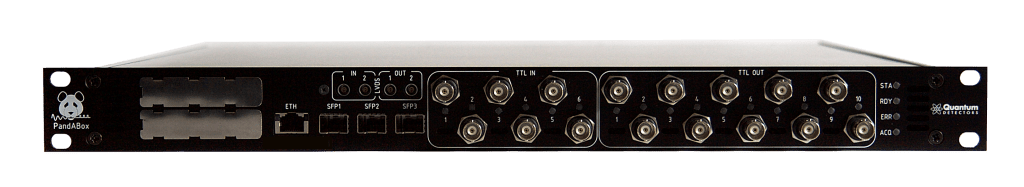
\includegraphics[width=0.7\textwidth]{dets/panda}


   XSpress3

   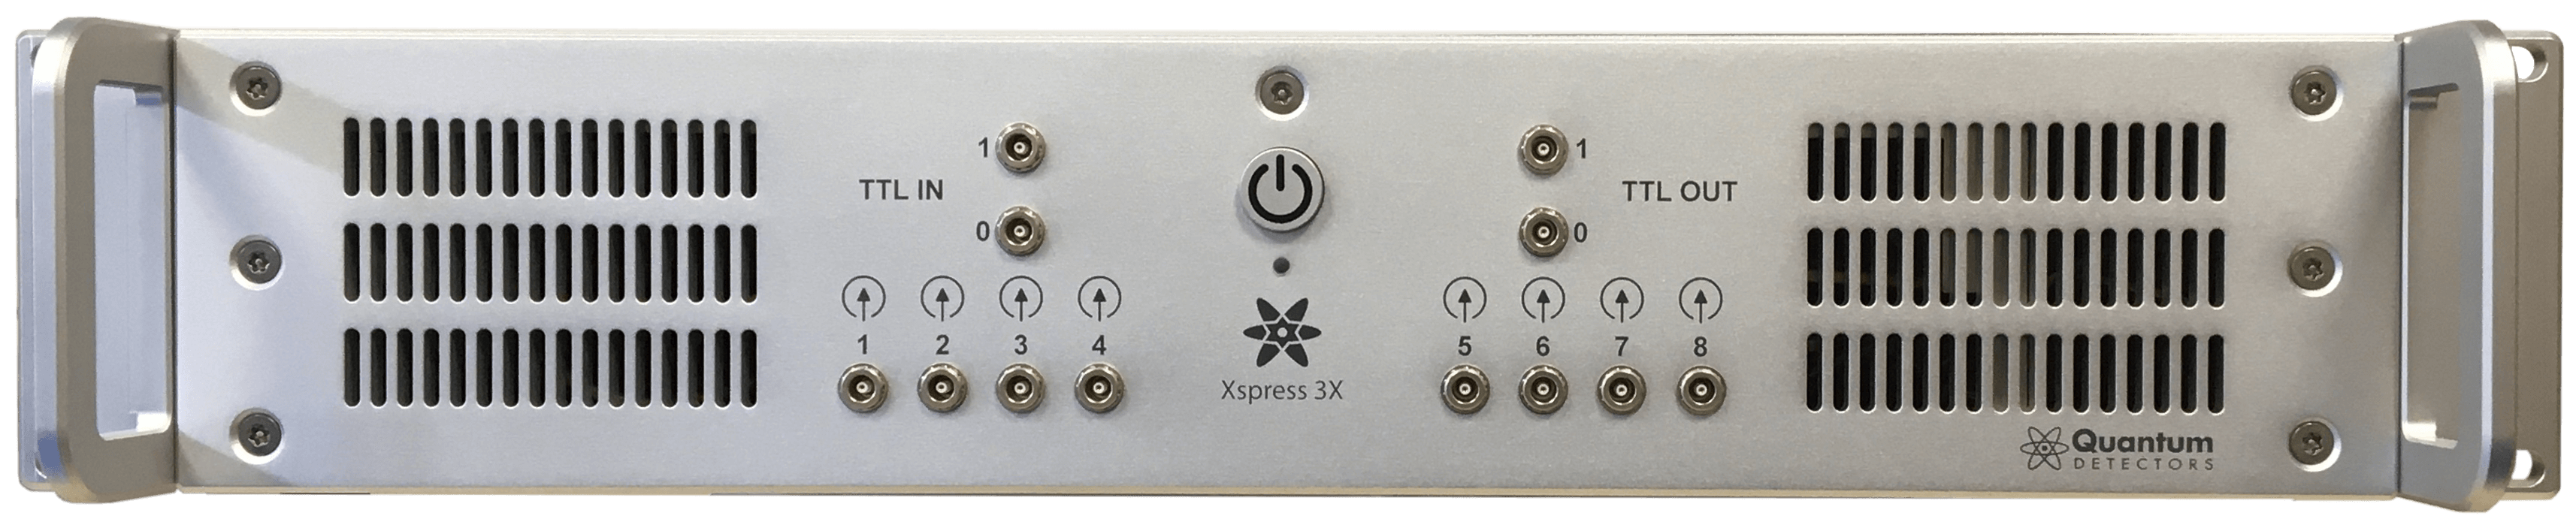
\includegraphics[width=0.7\textwidth]{dets/xspress}

   Basler

   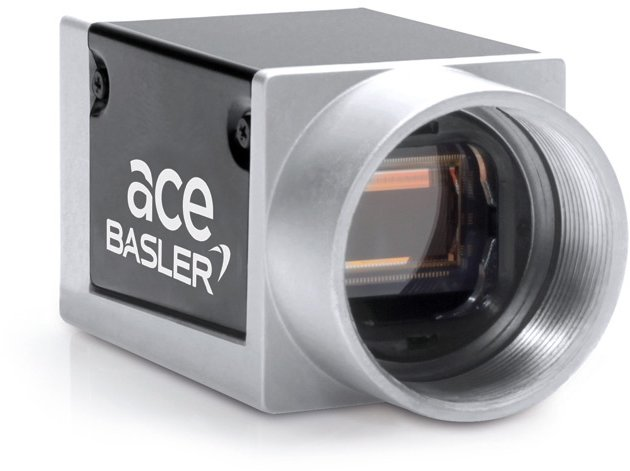
\includegraphics[width=0.5\textwidth]{dets/basler}

  AlbaEM
  \end{block}

\end{minipage}
\begin{minipage}[t]{0.49\textwidth}
\begin{block}{Software}
 \begin{itemize}
  \item Sardana
  \begin{itemize}
   \item Icepap
   \item Meta-data
   \item Filename
   \item Snapshots
  \end{itemize}

  \item Contrast
  \item Bluesky
 \end{itemize}
 \end{block}
\end{minipage}

\end{frame}

\begin{frame}{Event Formation}
 \centering
 \begin{minipage}{0.7\textwidth}
 \begin{tikzpicture}
  \node at (-2,0) {Detectors};
  %\node (det1) at (0,0) {\faCamera};
  %\node (mot) at (4,0) {\faSlidersH}; %\faCameraRetro};
  %\node (temp) at (6,0) {\faThermometerHalf};
  %\node (det2) at (2,0) {\faVideo};

  \node (det1) at (0,0) {\faCamera};
  \node (mot) at (4,0) {\faSlidersH}; %\faCameraRetro};
  \node (temp) at (6,0) {\faThermometerHalf};
  \node (det2) at (2,0) {\faCamera};

  \fill[white] (0,-0.5) rectangle (0.5,0.5);
  \fill[white] (2,-0.5) rectangle (1.5,0.5);

  \node at (-2,1) {Trigger Source};

  \node (panda) at (0,1) {\faWaveSquare};

  \draw[dotted] (panda) -- (det1);
  \draw[dotted] (panda) -- (det2.north);
  \draw[dotted] (panda) -- (mot.north);
  \draw[dotted] (panda) -- (temp.north);

  \node at (-2,-1) {Event Formation};
  \node (ef) at (3,-1) {\faHatWizard};

  \draw[very thick] (det1.south) -- (ef);
  \draw[very thick] (det2.south) -- (ef);
  \draw (mot.south) -- (ef);
  \draw (temp.south) -- (ef);


  \node at (-2,-2) {Analyses};
  \node (crop) at (3,-2) {\faCrop};

  \node (live) at (4,-2) {\faDesktop};

  \draw (crop) -- (live);

  \node at (-2,-3) {Reduced Recording};
  \node (file) at (3,-3) {\faFileArchive};
  \draw[line width=2mm] (ef) -- (crop);
  \draw[very thick] (crop) -- (file);
 \end{tikzpicture}
\end{minipage}
\begin{minipage}{0.29\textwidth}
\vspace{1cm}
 \begin{tabular}{rcccc}
   %$\stackrel{t}{\rightarrow}$ & ev 1 & ev 2 & ev 3 & ev 4 & ev 5 & ev 6 \\
   %\faCamera & \faImage & \faImage & \faImage & \faImage & \faImage & \faImage \\
   %\faVideo & \faCloudMoon & \faCloudMoonRain &  \faCloudShowersHeavy & \faCloudRain  & \faCloudSunRain & \faCloudSun \\
   %\faSlidersH & 0.5 &  & 0.6 &  & 0.5 & \\
   %\faTemperatureHigh &  & \faThermometerEmpty &  & \faThermometerHalf  &   & \faThermometerFull  \\

   $t \downarrow$  &\faCamera  &\faVideo  &\faSlidersH  &\faTemperatureHigh   \\
 e1  & \faImage  & \faCloudMoon  & 0.5  &   \\
 e2  & \faImage  & \faCloudMoonRain  &   & \faThermometerEmpty  \\
 e3  & \faImage  &  \faCloudShowersHeavy  & 0.6  \\
 e4  & \faImage  & \faCloudRain   &   & \faThermometerHalf   \\
 e5  & \faImage  & \faCloudSunRain  & 0.5     \\
 e6 & \faImage & \faCloudSun & & \faThermometerFull \\
  \end{tabular}

  \begin{block}{}
  \begin{itemize}
   \item non-uniform triggers
  \end{itemize}

 \end{block}
\end{minipage}


\end{frame}


\begin{frame}{Event Formation Bottleneck}
 \centering
 \begin{tikzpicture}
  \node at (-2,0) {Detectors};
  \node (det1) at (0,0) {\faCamera};
  \node (mot) at (4,0) {\faSlidersH}; %\faCameraRetro};
  \node (temp) at (6,0) {\faThermometerHalf};
  \node (det2) at (2,0) {\faVideo};

  \node at (-2,1) {Trigger Source};

  \node (panda) at (0,1) {\faWaveSquare};

  \draw[dotted] (panda) -- (det1);
  \draw[dotted] (panda) -- (det2.north);
  \draw[dotted] (panda) -- (mot.north);
  \draw[dotted] (panda) -- (temp.north);

  \node at (-2,-1) {Event Formation};
  \node (ef) at (3,-1) {\faHatWizard};

  \draw[very thick] (det1.south) -- (ef);
  \draw[very thick] (det2.south) -- (ef);
  \draw (mot.south) -- (ef);
  \draw (temp.south) -- (ef);


  \node at (-2,-2) {Analyses};
  \node[red] (crop) at (3,-2) {\faCrop};

  \node (live) at (4,-2) {\faDesktop};

  \draw (crop) -- (live);

  \node at (-2,-3) {Reduced Recording};
  \node (file) at (3,-3) {\faFileArchive};
  \draw[line width=2mm, red] (ef) -- (crop);
  \draw[very thick] (crop) -- (file);
  \pause
  \node at (3,-2) {
\includegraphics[height=3cm]{img/redis}};
 \end{tikzpicture}

\end{frame}

\begin{frame}{Existing Solutions}
\begin{minipage}[t]{0.49\textwidth}
 \begin{block}{Apache Flink} % \includegraphics[height=1cm]{img/flink.png}}
 \begin{itemize}
  \item exactly-once guarantee
  \item many small events
 \end{itemize}
 \end{block}

 \begin{block}{Hummingbird}
  \begin{itemize}
   \item XFEL development
   \item tailored to pulsed facilities
  \end{itemize}
 \end{block}
 \end{minipage}
 \begin{minipage}[t]{0.49\textwidth}
 \begin{block}{OnDA / HiDRA}
  \begin{itemize}
   \item DESY developments
   \item maintained?
  \end{itemize}

 \end{block}
 \begin{block}{EWOKS}
  \begin{itemize}
   \item large ecosytem
   \item data ingress from blissdata
  \end{itemize}

 \end{block}
 \end{minipage}

\end{frame}

\begin{frame}{Parallelisation by Event, not Stream (\texttt{map})}
 \centering
 \begin{tikzpicture}[xscale=1.4]
  \node at (-2,0) {Detectors};
  \node (det1) at (0,0) {\faCamera};
  \node (mot) at (4,0) {\faSlidersH}; %\faCameraRetro};
  \node (temp) at (6,0) {\faThermometerHalf};
  \node (det2) at (2,0) {\faVideo};

  \node at (-2,1) {Trigger Source};

  \node (panda) at (0,1) {\faWaveSquare};

  \draw[dotted] (panda) -- (det1);
  \draw[dotted] (panda) -- (det2.north);
  \draw[dotted] (panda) -- (mot.north);
  \draw[dotted] (panda) -- (temp.north);

  \node at (-2,-1) {Event Formation};
  \node (ef1) at (0,-1) {\faHatWizard};
  \node (ef2) at (2,-1) {\faHatWizard};
  \node (ef) at (5,-1) {\faHatWizard};

  \draw[very thick] (det1.south) -- (ef1);
  \draw[very thick] (det2.south) -- (ef2);
  \draw (mot.south) -- (ef);
  \draw (temp.south) -- (ef);


  \node at (-2,-3) {Analyses};
  \node (crop1) at (0,-3) {\faCrop};
  \node (crop2) at (1,-3) {\faCrop};
  \node (crop3) at (2,-3) {\faCrop};
  \node (crop4) at (3,-3) {\faCrop};
  \node (crop5) at (4,-3) {\faCrop};
  \node (crop6) at (5,-3) {\faCrop};
  \node (crop7) at (6,-3) {\faCrop};

  \node[below, text width=1cm, align=center] at (-1,-3.5) {$t \downarrow$};

  \node[below, text width=1cm, align=center] at (0,-3.3) {e3$\rightsquigarrow${\tiny r3}};
  \node[below, text width=1cm, align=center] at (1,-3.3) {e1$\rightsquigarrow${\tiny r1}};
  \node[below, text width=1cm, align=center] at (2,-3.3) {e5$\rightsquigarrow${\tiny r5}\\e8$\rightsquigarrow${\tiny r8}};
  \node[below, text width=1cm, align=center] at (3,-3.3) {e2$\rightsquigarrow${\tiny r2}\\e4$\rightsquigarrow${\tiny r4}};
  \node[below, text width=1cm, align=center] at (4,-3.3) {e9$\rightsquigarrow${\tiny r9}};
  \node[below, text width=1cm, align=center] at (5,-3.3) {e6$\rightsquigarrow${\tiny r6}};
  \node[below, text width=1cm, align=center] at (6,-3.3) {e7$\rightsquigarrow${\tiny r7}};


  \foreach \i in {1,2,...,7} {
    \draw (ef.south) -- (crop\i.north);
    \draw (ef1.south) -- (crop\i.north);
    \draw (ef2.south) -- (crop\i.north);
  };

 \end{tikzpicture}

 \begin{minipage}{0.49\textwidth}
\begin{block}{Balancing Constraints}
  \begin{itemize}
   \item event $2n$ and $2n+1$ to same worker
   \item event $m$ to worker \texttt{debug}
  \end{itemize}

 \end{block}
 \end{minipage}
 \begin{minipage}{0.49\textwidth}
 \begin{block}{Missing Inter Event Analysis}
  \begin{itemize}
   \item time integration
   \item long temporal correlations
  \end{itemize}

 \end{block}
  \end{minipage}

\end{frame}

\begin{frame}{Sequential Reduce}
 \begin{block}{Operations at Acquisition Speed}
  \begin{itemize}
   \item append to list
   \item sum
  \end{itemize}

 \end{block}

 \centering
 \begin{tikzpicture}
  \node at (-2,-1) {Event Formation};
  \node (ef1) at (0,-1) {\faHatWizard};
  \node (ef2) at (2,-1) {\faHatWizard};
  \node (ef) at (5,-1) {\faHatWizard};

  \node at (-2,-2) {Analyses};
  \node (crop1) at (0,-2) {\faCrop};
  \node (crop2) at (1,-2) {\faCrop};
  \node (crop3) at (2,-2) {\faCrop};
  \node (crop4) at (3,-2) {\faCrop};
  \node (crop5) at (4,-2) {\faCrop};
  \node (crop6) at (5,-2) {\faCrop};
  \node (crop7) at (6,-2) {\faCrop};

  \node at (-2,-3) {Reduce};
  \node (red) at (3,-3) {\faCog};

  \node[below left, text width=1cm, align=right] at (2.7,-3) {r1\\r2\\r3};


  \foreach \i in {1,2,...,7} {
    \draw (ef.south) -- (crop\i.north);
    \draw (ef1.south) -- (crop\i.north);
    \draw (ef2.south) -- (crop\i.north);
    \draw (crop\i.south) -- (red);
  };

  \node (live) at (5.5,-3.5) {\faDesktop};
  \node (web) at  (5.5,-4) {h5web};
  \node (silx) at (5.5,-4.5) {silx (2.2)};
  \node (hsds) at (4,-3.5) {HSDS};
  \draw (red) -- (hsds) -- (live);
  \draw (hsds) -- (web.west);
  \draw (hsds) -- (silx.west);

  \node at (-2,-4) {Reduced Recording};
  \node (file) at (3,-4) {\faFileArchive};

  \draw[very thick] (red) -- (file);


 \end{tikzpicture}

\end{frame}


\begin{frame}{Behind the Scenes}

 \begin{tikzpicture}[yscale=1]

  \node[color=title.fg, left] at (-1,-2) {wrapped(custom zmq)};
  \node[color=title.fg, left] at (-1,-4) {pickle in zmq};

  \node at (-2,-1) {Event Formation};
  \node (ef1) at (0,-1) {\faHatWizard};
  \node (ef2) at (2.5,-1) {\faHatWizard};
  \node (ef) at (5,-1) {
\includegraphics[height=1em]{img/crab}};

  \node (redis) at (7.5,-2) {
\includegraphics[height=1cm]{img/redis}};
   \node[below of=redis, yshift=-2mm, fill=white, text width=2cm, align=center] {batched truth};

  \node at (-2,-3) {Analyses};
  \node (crop1) at (0,-3) {\faCrop};
  \node (crop4) at (3,-3) {
\includegraphics[height=1.3em]{img/cpp}};
  \node (crop7) at (6,-3) {\faCrop};

  \foreach \i in {1,4,7} {
    \draw (ef.south) -- (crop\i.north);
    \draw (ef1.south) -- (crop\i.north);
    \draw (ef2.south) -- (crop\i.north);
  };

  \node at (-2,-5) {Reduce};
  \node (red) at (3,-5) {\faCog};


  \foreach \i in {1,4,7} {
    \draw (crop\i.south) -- (red.north);
  };

  \node[above of=ef2, yshift=-5mm, fill=white] {PULL};
  \node[above of=ef1, yshift=-5mm, fill=white] {SUB};
  \node[above of=ef, yshift=-5mm, fill=white] {PULL};


  \node[below of=ef1, yshift=5mm, fill=white] {ROUTER};
  \node[below of=ef2, yshift=5mm, fill=white] {ROUTER};
  \node[below of=ef, yshift=5mm, fill=white] {ROUTER};

  \node[above of=crop1, yshift=-5mm, fill=white] {\small DEALER};
  \node[above of=crop4, yshift=-5mm, fill=white] {\small DEALER};
  \node[above of=crop7, yshift=-5mm, fill=white] {\small DEALER};

  \node[below of=crop1, yshift=5mm, fill=white] {\small PUSH};
  \node[below of=crop4, yshift=5mm, fill=white] {\small PUSH};
  \node[below of=crop7, yshift=5mm, fill=white] {\small PUSH};

  \node[above of=red, yshift=-5mm, fill=white] {\small PULL};
 \end{tikzpicture}

\begin{minipage}[t]{0.49\textwidth}
\begin{block}{pytest}
  \begin{itemize}
   \item end-to-end scans
   \item includes \texttt{rust} component
  \end{itemize}
 \end{block}
\end{minipage}
\begin{minipage}[t]{0.49\textwidth}
 \begin{block}{Typing}
  \begin{itemize}
   \item MyPy
   \item Pydantic
  \end{itemize}

 \end{block}
\end{minipage}

\end{frame}

\begin{frame}{Performance Estimates}
K8s cluster of 10: dual Xeon\textsuperscript{\textregistered} Gold 6326, 100\,Gbit/s Mellanox SR-IOV, 465\,GB RAM
\begin{minipage}[t]{0.6\textwidth}

 %\begin{block}{Throughput}
 % 32KiB ZMQ Frames
 % 20KHz, mean 0.017376s, max 0.131092s
%\end{block}
% \begin{block}{DAQ cluster SRIOV 2MiB ZMQ frames}
% 2.6kHz, latencies mean 0.256980, max 0.356988 5GB/s
% \end{block}
% \end{minipage}
% \begin{minipage}[t]{0.59\textwidth}
%\begin{block}{End-2-End Dranspose}
 %2MB frames, 1500p/s
 %500kB frames, 5.5kHz, 2.7GB/s
 %128kB 12kHz
 %2KB frames, 13kHz

 \begin{tikzpicture}
 \pgfplotsset{set layers}
 \begin{semilogxaxis}[scale only axis,width=0.8\textwidth, height=0.5\textheight,axis y line*=left,xmin=32,log basis x={2},
  ylabel={k event/s}, xlabel={frame size (kB)},yticklabel style={/pgf/number format/fixed},xticklabels = {}]
   \addplot+[dashed, mark=x] coordinates {(2,13)
   (32,13)
   (131, 12.5)
   (320, 7.5)
   (512, 5.5)
   (720,4.1)
   (1280, 2)
   (1620, 1.9)
   (2048, 1.5)};
   \addplot+[dashed,  mark=x] coordinates {(2,11)
   (32,11)
   (131, 10)
   (320, 7)
   (512, 4.5)
   (720, 4)
   (1280, 1.8)
   (1620, 1.7)
   (2048, 1.2)};
   \addplot+[dashed,  mark=x] coordinates {
   (2,5.9)
   (32,7.5)
   (131, 7.2)
   (320, 5.7)
   (512,4.4)
   (1280,1.9)
   (1620, 1.5)
   (2048, 1.1)};
  \addplot+[dashed,  mark=x] coordinates {
  (2,4)
  (32,3.9)
   (131, 4)
   (320, 4)
  (512, 3.5)
  (720,2.7)
  (1280,1.5)
  (1620, 1.2)
   (2048, 0.9)};
  \end{semilogxaxis}
  \begin{semilogxaxis}[scale only axis,width=0.8\textwidth, height=0.5\textheight,xmin=32,log basis x={2},xticklabels = {32,64,128,256,512,1024,2048},
  legend columns=4,
 legend style={at={( 0.5,1.05)}, anchor=south},
  axis y line*=right,
  ylabel style = {align=center},
  ylabel={GB/s}]
   \addplot+[ mark=*] coordinates {(2,0)
   (32,0.6)
   (131, 1.8)
   (320, 2.4)
   (512, 2.8)
   (720,2.9)
   (1280, 2.5)
   (1620, 3.1)
   (2048, 2.8)};
   \addlegendentry{1 stream};
   \addplot+[ mark=*] coordinates {(2,0)
   (32,1.2)
   (131, 3.6)
   (320, 4.2)
   (512, 4.4)
   (720, 5.3)
   (1280, 4.8)
   (1620, 5.5)
   (2048, 4.8)};
   \addlegendentry{2 streams};
   \addplot+[  mark=*] coordinates {
   (2,0.25)
   (32,2.4)
   (131, 6.1)
   (320, 7.6)
   (512,9.2)
   (720,9)
   (1280,9.2)
   (1620, 9.6)
   (2048, 9.2)};
   \addlegendentry{4 streams};
   \addplot+[  mark=*] coordinates {
   (2,0.4)
   (32,4)
   (131, 12)
   (320, 12.8)
   (512, 14.4)
   (720,16)
   (1280,15.2)
   (1620, 16)
   (2048, 16)};
   \addlegendentry{8 streams};
  \end{semilogxaxis}
 \end{tikzpicture}
%\end{block}
 \end{minipage}
 \begin{minipage}[t]{0.39\textwidth}
 \hfill
  \begin{tikzpicture}
\begin{axis}[
    width=\textwidth, height=0.66\textheight,
    xlabel={E2E Latency (ms)},
    area style,xmin=0,
    legend style={at={( 0.5,1.05)}, anchor=south},
    ]
\addplot+[ybar interval,mark=no] plot coordinates { (0.7060000000000001, 72.0) (0.8237000000000001, 119.0) (0.9414, 51.0) (1.0591, 37.0) (1.1768, 16.0) (1.2945000000000002, 3.0) (1.4122, 1.0) (1.5299, 2.0) (1.6476000000000002, 0.0) (1.7652999999999999, 0.0) (1.883, 0.0) (2.0007, 0.0) (2.1184, 0.0) (2.2361, 0.0) (2.3538, 0.0) (2.4715000000000003, 0.0) (2.5892, 0.0) (2.7069, 0.0) (2.8245999999999998, 0.0) (2.9423, 0.0) (3.06, 0.0) (3.1776999999999997, 0.0) (3.2954, 0.0) (3.4131, 0.0) (3.5307999999999997, 0.0) (3.6485, 0.0) (3.7662, 0.0) (3.8839, 0.0) (4.0016, 0.0) (4.1193, 1.0) };
\addlegendentry{2kB frames};
\addplot+[ybar interval,mark=no, dashed] plot coordinates { (1.91, 16.0) (2.0208666666666666, 44.0) (2.131733333333333, 53.0) (2.2426, 58.0) (2.3534666666666664, 52.0) (2.4643333333333333, 21.0) (2.5751999999999997, 21.0) (2.6860666666666666, 8.0) (2.796933333333333, 11.0) (2.9078, 1.0) (3.0186666666666664, 1.0) (3.129533333333333, 1.0) (3.2403999999999997, 1.0) (3.3512666666666666, 2.0) (3.462133333333333, 2.0) (3.5729999999999995, 3.0) (3.6838666666666664, 1.0) (3.7947333333333333, 0.0) (3.9055999999999997, 1.0) (4.016466666666666, 2.0) (4.127333333333333, 0.0) (4.2382, 0.0) (4.349066666666666, 2.0) (4.459933333333333, 0.0) (4.570799999999999, 0.0) (4.681666666666667, 0.0) (4.792533333333333, 0.0) (4.9033999999999995, 0.0) (5.014266666666666, 0.0) (5.125133333333333, 1.0) };
\addlegendentry{2MB frames};
\end{axis}
\end{tikzpicture}
 \end{minipage}
limits on around \textbf{2\,GB/s} per stream or \textbf{12\,kHz} at a \textbf{few ms}
\end{frame}




\begin{frame}{Development: Testing}
 \begin{block}{Recording}
 \begin{itemize}
  \item ingesters optionally write all streams to disk (sequential cbor dumps)
  \item common experimental setup
 \end{itemize}



 \end{block}

\begin{block}{Replay}
\begin{itemize}
 \item from recorded stream dumps
 \item from hdf5 files
\end{itemize}
\end{block}

\begin{block}{Local}
 run file-based ingesters, workers and reducer locally
\end{block}

\end{frame}



\begin{frame}{Case Study: NanoMAX}
\begin{minipage}{0.6\textwidth}
  \begin{block}{Sources}
   \begin{itemize}
    \item XSpress3
    \item Contrast (Motor Positions)
   \end{itemize}
  \end{block}

  \begin{block}{Analysis / Output}
   \begin{itemize}
    \item PyMCA fluorescence fitting
    \item Concentration Map
   \end{itemize}
  \end{block}

\end{minipage}
\begin{minipage}{0.39\textwidth}
 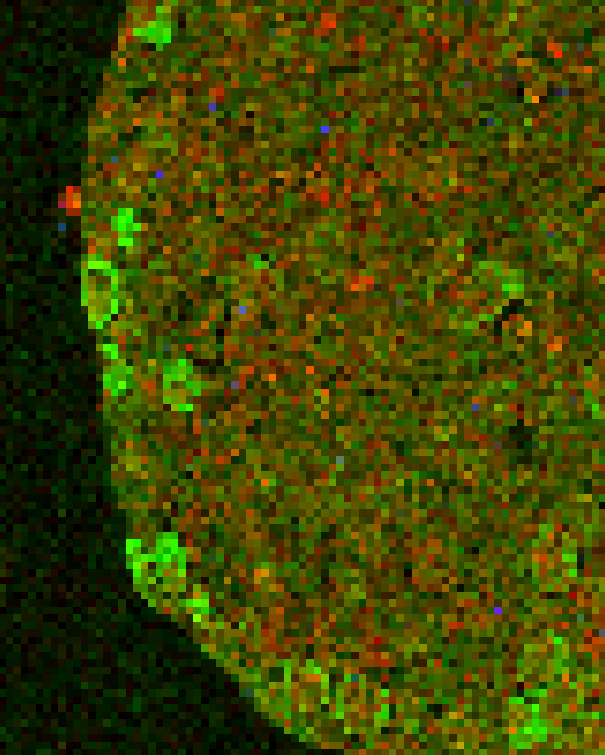
\includegraphics[width=\textwidth]{img/xrf}
\end{minipage}

\end{frame}

\begin{frame}{Case Study: DanMAX}
 \begin{tabularx}{\textwidth}{rm{3cm}cccl}
 Sardana & Basler & Pilatus & Orca & PandAbox &\\
  \multicolumn{2}{c}{Beam CoG,
    Beam Alignment}
    & & & & \raisebox{-0.5\totalheight}{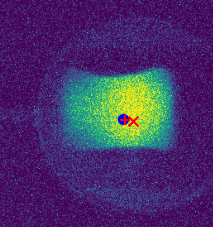
\includegraphics[width=1.5cm]{img/beamcog} } \\
  & & Pileup File & & & \raisebox{-0.5\totalheight}{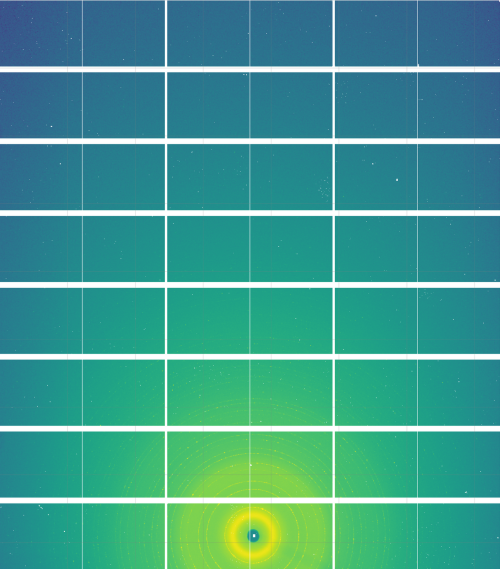
\includegraphics[width=1.5cm]{img/pileup}} \\
  & & & \multicolumn{2}{c}{Encoder angle} & \raisebox{-0.5\totalheight}{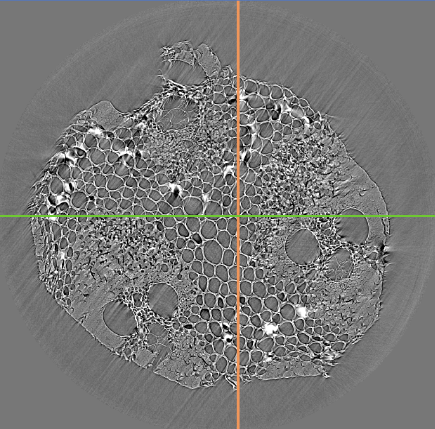
\includegraphics[width=1.5cm]{img/tomo}} \\
 \end{tabularx}
\end{frame}


\begin{frame}
 \centering
 \Huge \usebeamercolor[fg]{title} \texttt{python -m pip install dranspose}
 \medskip
\Huge \usebeamercolor[fg]{title} \texttt{docker-compose, helm}
\bigskip

 https://dranspo.se
\bigskip

{\large or come to Max IV, we are hiring: paul.bell@maxiv.lu.se}
\end{frame}


\end{document}
